\chapter{调制识别的深度框架研究}
\section{引言}

有几种完善的网络体系结构,包括多层感知器,卷积网络的许多变体以及循环网络。
 尽管机器学习的目标是开发通用技术,但目前最先进的网络类型似乎仍然是特定于应用程序的。 例如,谷歌认为卷积长短期深度神经网络(CLDNN)值得申请专利,尽管它只用于他们的语音处理研究。 
 图像识别领域的最新技术采用了初始架构,残留网络和其他允许卷积层组合的体系结构的变体,
 同时管理权重和激活的组合复杂性。 \par

我们将深度神经网络应用到无线电调制识别任务中,研究机器学习的最新进展。 结果表明,无线电调制识别不受网络深度的限制,进一步的工作应着重于提高学习的同步和均衡。 这些领域的进步可能来自为这些任务设计的新架构或通过新颖的培训方法。\par

在将深度神经网络应用于无线通信信号之前,值得回顾其他应用领域的现状。下一节将回顾深度神经网络架构和学习进展,这些进展可能对无线通信应用是有效的和有用的。在回顾有趣的深层架构和训练方法之后,结果在第三部分和第四部分讨论。 \par

\subsection{卷积神经网络}

在所有现有技术深度神经网络中的共同元素是卷积层的使用。卷积层由Nf卷积滤波器组成。图像和手写识别开始使用卷积图层来提供特征平移不变性[8]。对于已经熟悉FIR滤波器和DSP的人来说,神经网络中卷积滤波器的使用可能与预期略有不同,至少部分原因是由于神经网络中的激活函数的使用。神经网络中的卷积通常非常小(1x1到5x5是图像处理中的常见尺寸)。在典型的DSP应用中,滤波器非常宽(很多分支/高阶)而非深度(小分支,但是级联)。实现这些滤波器的现代方法(例如多相滤波器组)通常提供了用于由于计算或等待时间原因而减小滤波器宽度的方法。标准卷积层[9]的传递函数在等式3中给出,其中yi是第i个滤波器的输出特征图,b和k代表学习偏差和滤波器权重参数,xi代表输入激活,?表示卷积运算,并且f(::)表示诸如整流线性单元(ReLU)或S形的(通常非线性的)激活函数。。\par

图像处理的神经网络的一个明显趋势是建立更深的网络来学习更复杂的功能和层次特征关系[2],[1]。
深度网络使得可以从原始数据中更容易地学习更复杂的功能,而不是使用相同数量参数的浅层网络[1],[18];
然而,人们普遍认为神经网络中的深度受不稳定梯度的限制,不稳定梯度在网络中的早期层或后期层中爆炸或消失。
近年来,通过在优化器中使用梯度归一化以及不会加剧消失梯度问题的非线性(如整流线性单位(ReLU)),
近年来该问题得到了改善。因此,几个重要的架构已被用于赢得竞争,如ImageNetby增加深度,
我们将着眼于提高无线电调制识别。\par

\subsection{GoogLenet}
GoogLenet [17]中使用的初始架构是一种成功的方法,可以提高网络深度,并能够将不同规模的特性推广到一般管理复杂性。
该网络由重复启动模块组成。每个启动模块(如图1所示)包含四条并行路径,输出是四个并行输出的串联。
第一条路径是一组沿着选定信息转发的1x1卷积。
1x1卷积是一种选择性高速公路网络,它只是简单地向前传递信息而不进行变换。
第二和第三路径是1×1卷积,接着是一组3×3和5×5卷积以提供多个比例的特征检测。
最后,最后的平行路径是一个3x3池化层,接着是1x1卷积。
网络中的中间启动模块连接到softmax分类器,这会导致网络全球培训损失。
这些分类器被认为有助于防止消失梯度。\par

\subsection{ResNet}
增加深度的另一种方法是使用跨层转发信息的体系结构。
迄今为止赢得ImageNet 2015的最佳方法是残余网络[4]。
剩余网络将一层的输出添加到更深层的两层输出中(如图2所示)。
这被称为残留网络,因为转发的信息迫使网络学习残差函数作为特征提取的艺术。 
剩余网络作者认为消失梯度可以通过广泛采用的归一化技术来解决,而深度网络的深度则受限于深度网络的训练复杂度,
这可以通过残差函数来简化。\par


\subsection{CLDNN}
CLDNNs是一种语音处理方法,它可以在原始时域波形上进行操作,而不是专家语音功能,如log-mel cepstrums [16],[15]。 该体系结构使用两个卷积层,随后是两个由长期短期内存(LSTM)单元组成的循环层。 LSTM是一种常见的经常性网络架构,由几个门控制,历史维持多久[5]。 CLDNN也可以具有绕过层的连接,旨在为提取的功能提供更长的时间上下文。 例如,原始CLDNN在LSTM层之前转发具有卷积层输出的原始样本[15]。\par

受使用专业知识指导网络体系结构(如卷积网络和CLDNN)的启发,我们尝试使用卷积网络,我们将其称为卷积匹配滤波器。 相当简单的想法是采用典型通信接收器的通用架构,并构建具有类似部分的神经网络架构。 通信接收机有一个滤波器(通常是采样器),通常前置滤波器抽取每个符号的少量采样,用于执行相移以找到最佳采样点的同步器,然后采样器切片成比特或发射音频以进行模拟调制 。与此类似的神经网络体系结构是一个卷积层,后面跟着一个LSTM。\par


\section{结果及分析}

\subsection{神经网络训练}

网络的超参数(如学习速率,每层过滤器/特征映射的数量,过滤器大小以及某种程度上的层数)都会影响网络规模并且难以优化。 最近的研究尝试将超参数优化为可以用反向传播和梯度下降(如网络权重和偏差)进行训练的常规参数。 对于这项研究,我们忽略训练超参数,并使用adam优化器[6],它提供梯度归一化和动量,降低超参数的重要性,如学习率。

在工作的指导下,深度比特征图的数量更重要[2],我们将建立一个类似于无线电卷积调制网络[13]中使用的基线卷积网络。 我们的第一步是调整每个滤波器的滤波器数量和抽头数量,并将其视为不重要的超参数,用于余下的实验以测试不同架构对RF数据的适用性。

\subsection{网络参数}

网络的超参数(如学习速率,每层过滤器/特征映射的数量,过滤器的大小以及层的数量)都会影响网络规模,难以优化。
最近的研究尝试将超参数优化为可以用反向传播和梯度下降(如网络权重和偏差)进行训练的常规参数。
对于这项研究,我们忽略训练超参数,并使用adam优化器[6],它提供了梯度归一化和动量,降低了像学习率这样的超参数的重要性。
在工作的指导下,深度比特征图的数量更重要[2],我们将建立一个类似于无线电卷积调制网络[13]中使用的基线卷积网络。
我们的第一步是调整每个滤波器的滤波器数量和抽头数量,并将其视为不重要的超参数,用于剩余的实验,
以测试不同架构对RF数据的适用性。\par

我们使用RadioML2016.10a数据集[12]作为评估调制识别任务的基础。
目标是使用128个样本的复数(基带I / Q)时域矢量来识别11种可能类别中的调制方案。 
128个样本以2x128向量馈入网络,其中复数时间样本的实部和虚部被分开。
该数据集使用功率延迟分布,频率选择性衰落,本地振荡器偏移和加性高斯白噪声以及这些效应的细节[12]。
数据集标有调制类型和SNR地面实况。
我们使用全SNR的top-1分类精度作为单个数字基准,并且比较技术显示SNR高于1的精度。
所有模型和培训均使用Kera深度学习库,使用Nano GTX 1070 GPU使用theano后端。
我们从一个类似于CNN2网络的网络开始[13]。
这是选择的基线,因为[13]的结果显示专家方法的显着改进;任何进一步的改进都应该被认为是最先进的。
主要区别在于我们将在每个图层上使用尺寸为1xtaps的nfilt滤镜。
我们将做一个简单的超参数优化\par

\begin{enumerate}
	\item[a.] 为RF调制识别找到最佳滤波器数量和滤波器大小
	\item[b.] 从网络深度和过滤器大小的其他领域获得测试假设
\end{enumerate}

\subsection{基准卷积网络}

基线卷积网络在softmax分类器之前有两个卷积层和一个致密层。每个隐藏层具有整流线性单元(ReLU)激活功能和50%的丢失。第一个超参数优化是卷积层的大小。每个图层都会有1x3的过滤器,我们将改变过滤器的数量以找出需要的数量。从[1],[18],[2]我们预计在过度配合发生之前,过滤器数量的较大范围会带来类似的性能。\par

正如预期的那样,每层大约有30到70个过滤器,而且性能非常相似,这个窗口相当大。图10显示了10-滤波器增量的20-90滤波器的前1类分类精度。对于其余的实验,我们将使用每层50个滤波器。接下来,我们优化每个过滤器的大小。 [2]表明,滤波器的大小也有最小的影响,但基于无线电领域和数据集的专业知识,我们预期8抽头滤波器是最优的。对于这个实验,我们使用一个具有单个隐藏密集层的双卷积层网络,接着是softmax分类器。卷积层每个都有50个滤波器,滤波器大小为1xntaps,其中ntaps从3到12变化。。\par

\begin{figure}[!h]
	\centering
	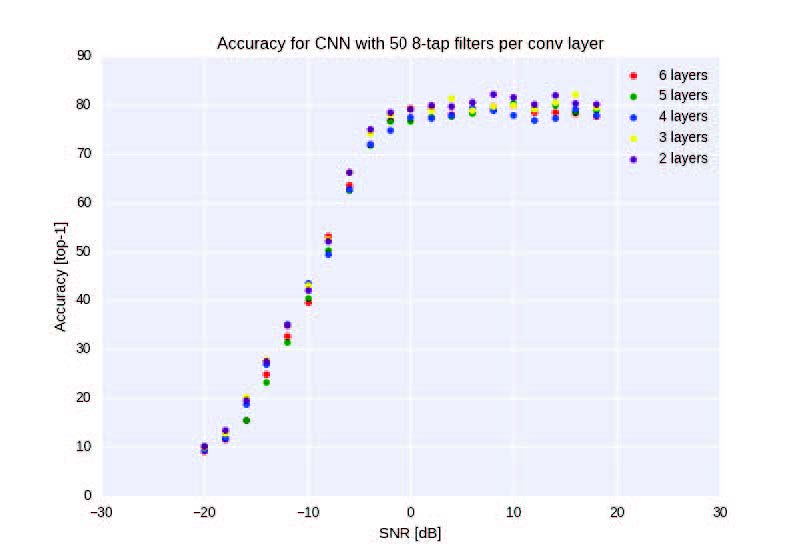
\includegraphics[scale=1]{figures/chapter_5/fig3}
	\caption{改变每层滤波器的数量具有较小的影响,在更高的SNR下更明显。
		每个网络在2个卷积层网络中都有1x3个过滤器,并有1个致密层和一个softmax分类器。}
\end{figure}

每个卷积层的滤波器尺寸变化的结果表明,较小的滤波器不如较大的滤波器。 我们根据数据集的专家知识假设8抽头滤波器是最好的。 图4中每个SNR图的结果很难区分清楚的赢家; 然而,整个数据集的分类准确性表明,7-12次水龙头都具有相似的性能约61%,差异在统计上不显着。\par

\begin{figure}[!h]
	\centering
	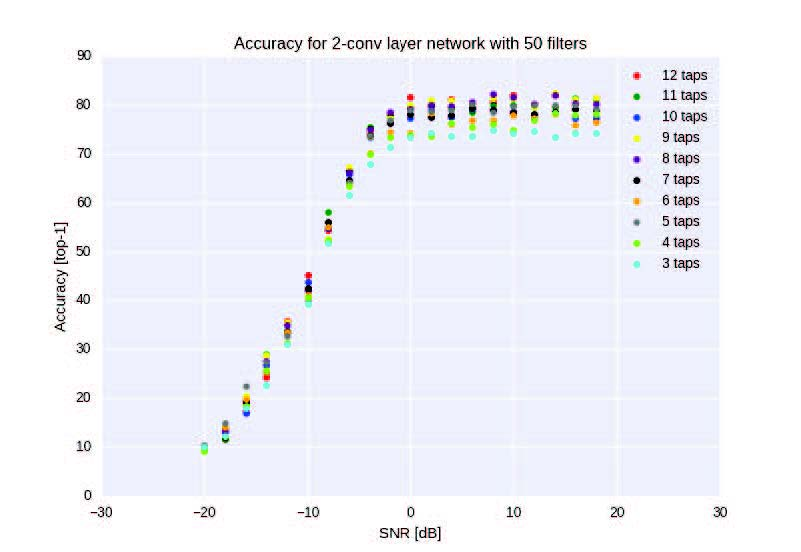
\includegraphics[scale=1]{figures/chapter_5/fig2}
	\caption{改变DNN中卷积层的数量不会改进无线电调制识别。}\label{fig_5_2}
\end{figure}

最后,对于纯卷积网络,我们尝试增加网络深度。对于这个实验,我们使用带1x8滤波器的50抽头卷积层。卷积层之后,我们使用一个隐藏的密集层,然后使用最后一个密集的softmax分类器。我们从一个2卷积层网络开始,并添加卷积层。深度学习的趋势表明,增加更多图层应该会改善分类性能,直到渐变变得不稳定。\par


\begin{figure}[!h]
	\centering
	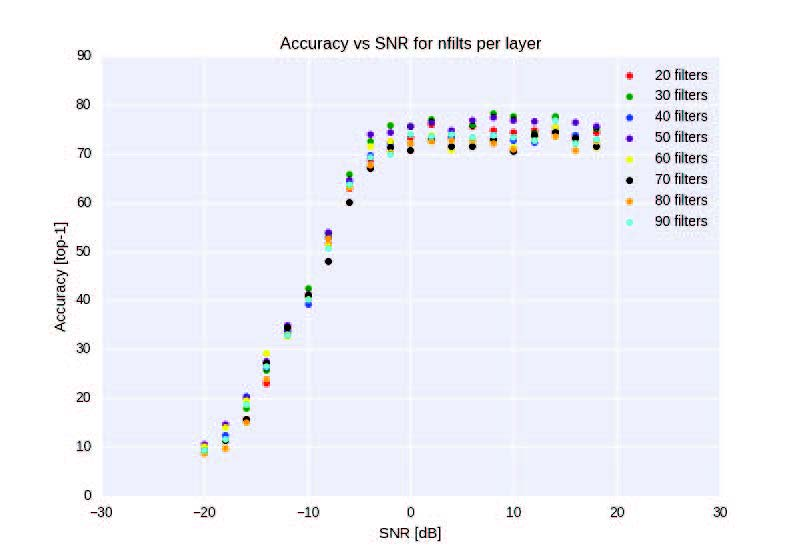
\includegraphics[scale=1]{figures/chapter_5/fig1}
	\caption{改变两个卷积层中的抽头数量(滤波器大小),较低的水龙头数量明显较差,
		但性能集群随水龙头数量的增加而增加。}\label{fig_5_1}
\end{figure}

改变卷积层的数量在分类准确性方面几乎没有改善。图5显示了该任务的信噪比精度。这表明我们的网络没有更多的特征深度可以学习。由于调制数据通常只改变复数正弦曲线的幅度,频率或相位,因此数据的起始层次不高;然而,令人惊讶的是,添加更多的卷积层似乎并不能在较低的信噪比下帮助降低噪声的影响。\par

\subsection{残留网络}
尽管添加更多卷积层不会提高分类准确性并不奇怪,但令人惊讶的是,分类和丢失只要2或3卷积层即可达到平稳。 最初的研究结果表明,较深的网络会导致较高的训练损失,这表明较高的训练难度而不是过度训练。 图6显示,我们的超参数优化CNN和9层残留网络达到了相似的损失,验证损失和未显示的准确性; 然而,剩余网络在更少的时期学习。 我们还试验了5-9层的残留网络,它们都具有相似的性能和训练时间。 这与我们针对普通CNN深度的超参数搜索相结合,表明我们不受无线电学习任务网络深度的限制,尽管我们受限于纯粹CNN架构可以学习的功能。\par

\begin{figure}[!h]
	\centering
	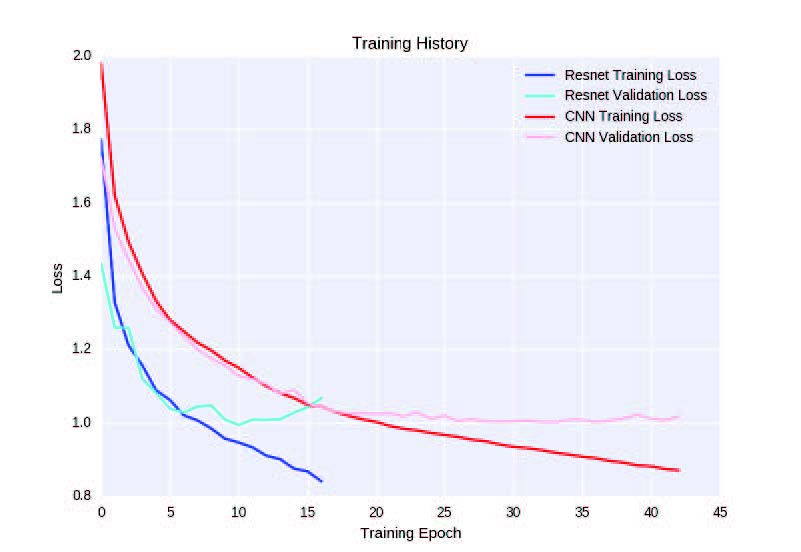
\includegraphics[scale=1]{figures/chapter_5/fig4}
	\caption{显示超参数优化的CNN和9层残留网络的训练损失和验证损失的训练历史记录}
\end{figure}
\par

\subsection{InceptionModel}
先启模块在我们的实验中也没有改进无线电调制分类,使用为我们的数据集调整的初始模块。 每个模块使用的三个分支是50个1x1滤波器,50个1x3滤波器和50个1x8滤波器。 1x3和1x5滤波器分支前面也有50个1x1滤波器,如图7所示。网络中1-4个启动模块的结果并没有显示出我们的超参数优化CNN的改进。 同样,这表明我们不受深度的限制,也不受限于滤波器的规模。\par

\begin{figure}[!h]
	\centering
	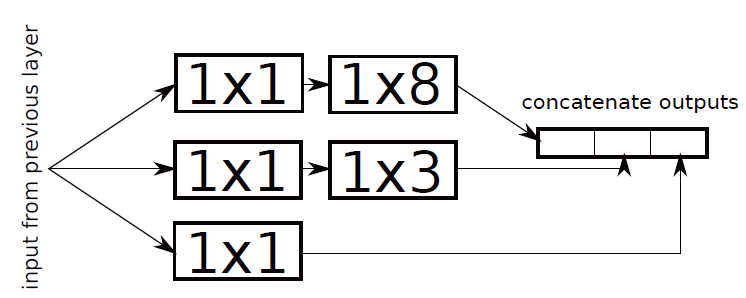
\includegraphics[scale=1]{figures/chapter_5/fig5}
	\caption{用于显示卷积滤波器尺寸的RF数据的初始模块。 每个卷积层有50个过滤器}
\end{figure}

\subsection{CLDNN}

作为我们测试的最终架构添加了经常性网络层,即那些由LSTM单元组成的层,用于对时间特征进行建模。 这种方法广泛用于时间序列应用,我们预计调制基带时间序列可能同样适用。 我们测试了两层和三层卷积,然后在CLDNN类型体系结构中重复出现层,在重复层之前有和没有前向/旁路连接。 我们发现前向连接作为原始波形和卷积输出的连接,如图8所示,与其他体系结构相比,分类精度更高,梯度下降更稳定。 使用会创建类似前面描述的卷积匹配滤波器检测器的体系结构的合并层不利于分类。\par
\begin{figure}[!h]
	\centering
	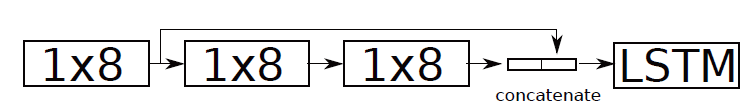
\includegraphics[scale=1]{figures/chapter_5/fig6}
	\caption{用于RF数据的CLDNN体系结构。 在进入LSTM之前,第一个1x8卷积层的输出与三个1x8卷积层的输出级联。}
\end{figure}

为了进一步理解什么限制了分类精度,我们查看了图10中所示的CLDNN的混淆矩阵。有两个主要混淆领域。 一个在模拟调制之间,另一个在高阶QAM之间。 模拟调制将很难解决,但是QAM可以通过更好的同步和减少信道损伤来改善。\par

\begin{figure}[!h]
	\centering
	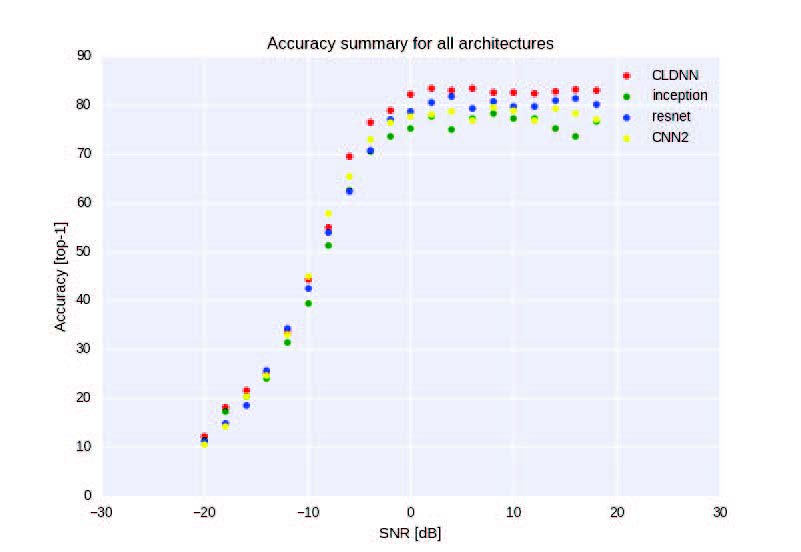
\includegraphics[scale=1]{figures/chapter_5/fig7}
	\caption{CLDNN的信噪比始终优于其他网络架构,信噪比高于-8dB}
\end{figure}

为了进一步理解什么限制了分类的准确性,我们看一下图8所示的CLDNN的混淆矩阵。有两个主要的混淆领域。一个在模拟调制之间,另一个在高阶QAM之间。模拟调制将很难解决,但是QAM可以在更好的同步和减少信道损伤的情况下得到改善。\par

\begin{figure}[!h]
	\centering
	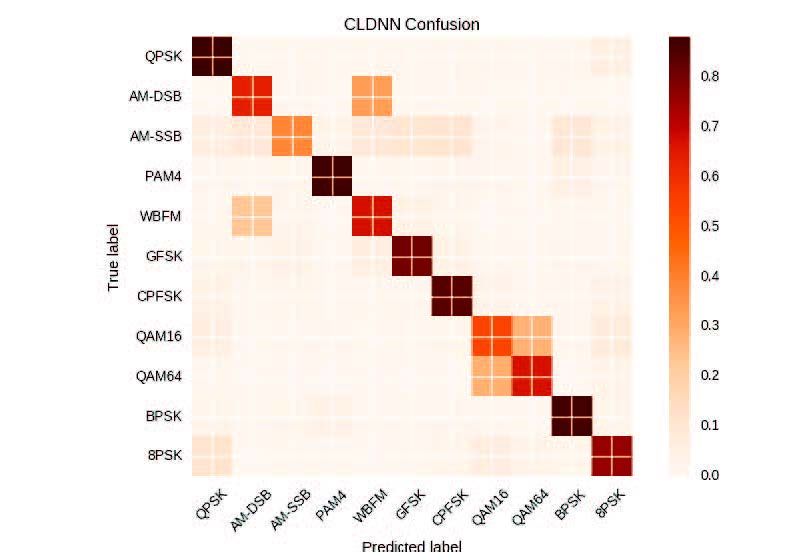
\includegraphics[scale=1]{figures/chapter_5/fig8}
	\caption{CLDNN的全SNR混淆矩阵显示了模拟调制和高阶QAM之间单独混淆之间最混乱的问题。}
\end{figure}

对CLDNN在每一层学习的内容有直觉,对指导未来的工作很重要。 为此,我们绘制了一些滤波器抽头的时间和频率表示。 对于频率响应,滤波器抽头用零填充100个零点以获得128点FFT。图 图11a和12a示出了来自第一层的两个选择滤波器。 专家的眼睛看起来并不特别熟悉时域表示; 然而频率响应确实显示出成形的低通滤波器。 未示出的其他滤波器具有频率选择性组件,DC阻断器和类似sinc的频谱形状。\par
\begin{figure}[!h]
	\centering
	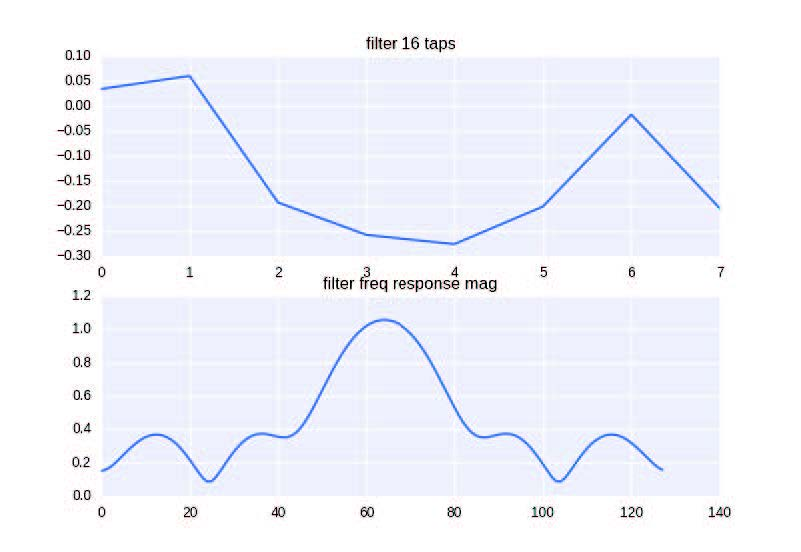
\includegraphics[scale=1]{figures/chapter_5/fig9_a}
	\caption{我们训练的CLDNN的第一卷积层中滤波器的时间和频率幅度表示。。}
\end{figure}
\begin{figure}[!h]
	\centering
	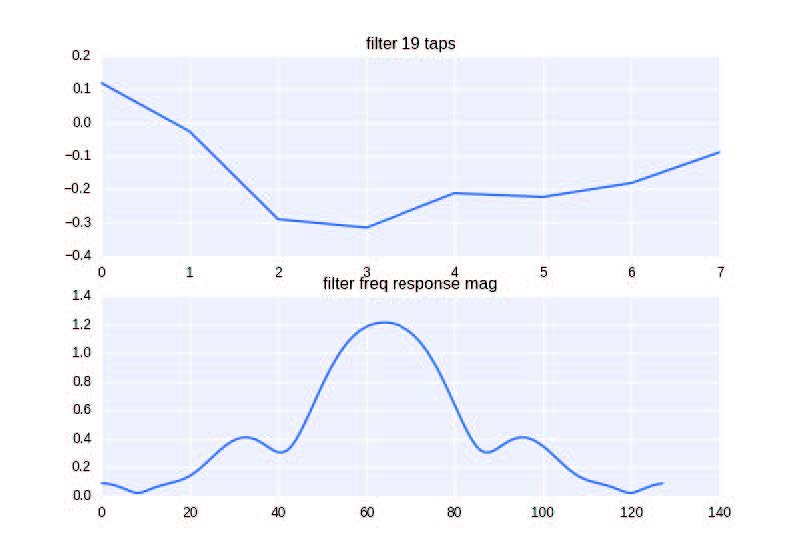
\includegraphics[scale=1]{figures/chapter_5/fig10_a}
	\caption{我们训练的CLDNN的第一卷积层中滤波器的时间和频率幅度表示。。}
\end{figure}
另一种可视化这些滤波器的方法是将随机数据应用于它们,并对特定滤波器的输出执行梯度上升,该滤波器将收敛到最能激活卷积神经元的数据上[11]。 选定的两个过滤器的结果如图2所示。 11b和12b。 所得到的载体看起来有点像粗PSK和FM / FSK调制到专家眼睛。 由于模拟的信道模型,矢量还显示出存在于我们的数据集中的一些恒定的相位旋转。 需要注意的是,选择这两种过滤器可视化并非所有过滤器都对专家有意义。\par

\begin{figure}[!h]
	\centering
	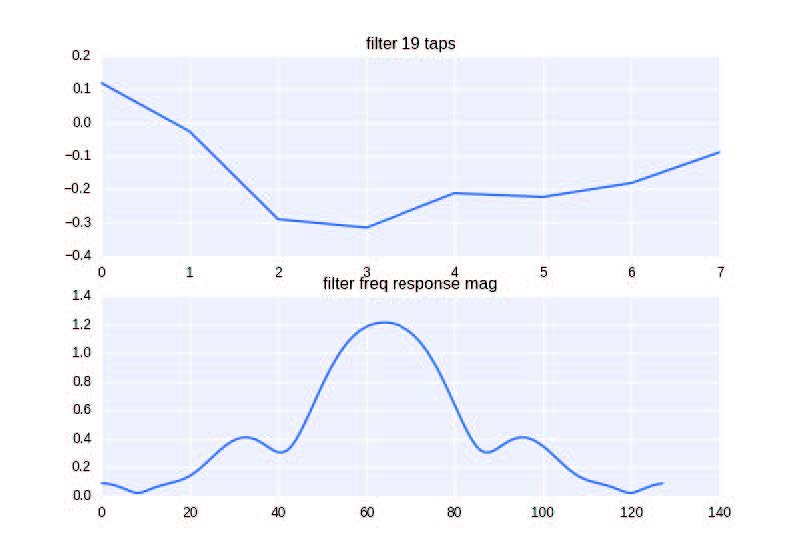
\includegraphics[scale=1]{figures/chapter_5/fig9_b}
	\caption{随机数据训练最大程度地激活过滤器,看起来像BPSK。}
\end{figure}
\begin{figure}[!h]
	\centering
	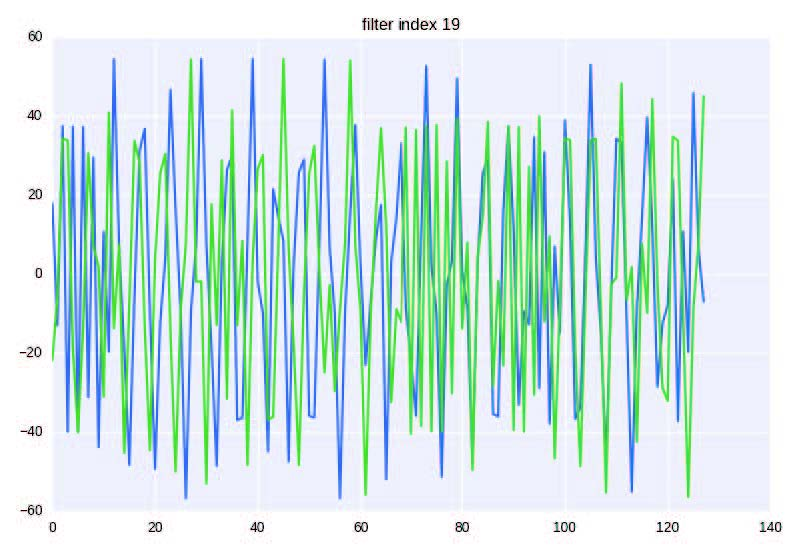
\includegraphics[scale=1]{figures/chapter_5/fig10_b}
	\caption{训练最大程度激活滤波器的随机数据,这看起来像FM或FSK调制。}
\end{figure}


\section{本章小结}
深度神经网络在无线电领域的性能似乎不受网络深度的限制,就像图像,自然语言处理和声学领域一样。 虽然我们的实验将调制识别作为基准任务,但我们期望其他无线机器学习任务能够使用类似的网络架构。 无线电任务深度学习的进一步发展可能来自改进的训练方法和网络架构,这些架构可以学习转换射频数据以消除无线信道的影响,而这些神经网络架构并非为此设计的。 目前正在探索的一个例子是使用空间变换来均衡和同步输入波形[14]。\par

这些实验还着重于名义上带宽归一化的数据集,这是对从真实无线电传输中捕获的信号的不良假设。 将来在实际应用中使用的网络需要学习对信号进行重新采样以获得带宽规格化,或者学习许多带宽的特性。 可重新采样,同步和消除非线性信道失真的网络都是该领域未来令人兴奋的工作。 我们相信,随着无线电环境变得越来越复杂,将调制,多调制协议的不同时间行为和多个无线电发射机组合在一个频带内进行互操作,这些深层网络中的层次结构的许多概念将越来越重要,使我们的网络 可以有效地应对复杂性,正如在复杂的多物体场景中的视觉域中所显示的一样。\par